% вторая часть

\section{Восстановление глубины из одного расфокусированного изображения}

Рассмотрим сложную задачу восстановления глубины из одного расфокусированного изображения. Входное расфокусированное изображение повторно размыто с использованием гауссова ядра, а значение размытости размытия может быть получено из коэффициента градиента между входными и повторно размытыми изображениями. Распространяя количество размытия в крайних положениях на все изображение, можно восстановить всю карту глубины сцены.

Результат восстановления глубины нашего метода. (рисунок~\ref{fig:input}) Большая интенсивность означает большую глубину на всех картах глубины

\begin{figure}[H]
	\centering
	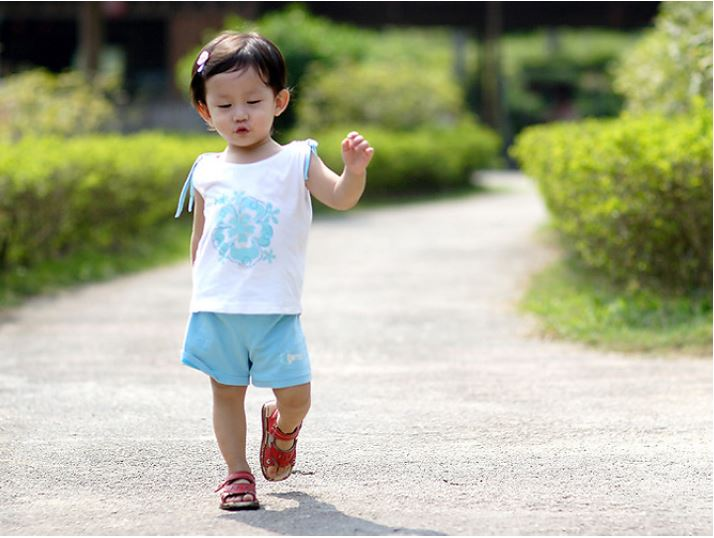
\includegraphics[width=0.4\linewidth]{pics/input}
	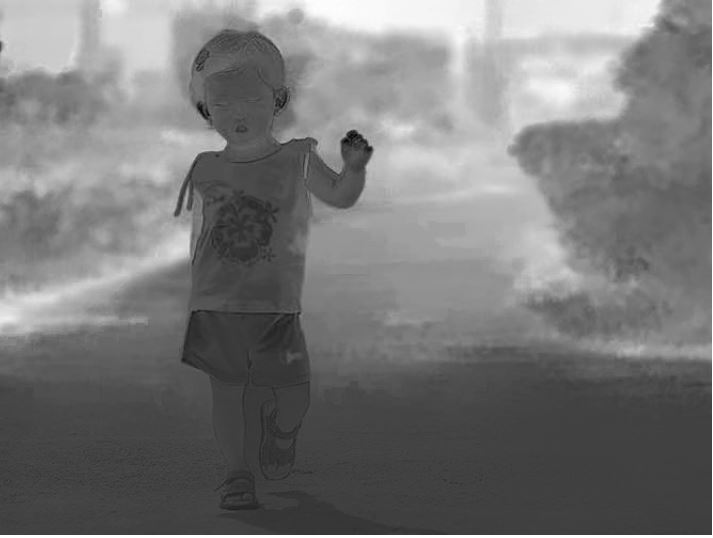
\includegraphics[width=0.4\linewidth]{pics/depth_map}
	\caption{Входное изображение и карта глубины}
	\label{fig:input}
\end{figure}

Сосредоточимся на более сложной проблеме восстановления относительной глубины из одного расфокусированного изображения, захваченного некалиброванной обычной камерой. Метод обратной диффузии~\cite{Proc} моделирует размытие дефокусировки в качестве процесса диффузии тепла и использует неоднородную диффузию тепла для оценки размытости размытия в краевых положениях. В отличие от этого, моделируем размытие дефокусировки как размытие 2D Gaussian. Входное изображение повторно размывается с использованием известного гауссовского размытия, и рассчитывается коэффициент градиента между входными и повторно размытыми изображениями. Величина размытия в краевых местоположениях может быть получена из отношения.

Рассмотрим эффективный метод оценки размытия, основанный на гауссовском градиентном соотношении, и показываем, что он устойчив к шуму, неточному расположению краев и помехам от соседних ребер. Без каких-либо изменений в камерах или при использовании дополнительного освещения наш метод позволяет получить карту глубины сцены, используя только одно расфокусированное изображение, снятое обычной камерой. Как показано (рисунок~\ref{fig:input}), этот метод может извлекать карту глубины сцены с довольно высокой степенью точности.

\subsection{Модель дефокусировки}

Оцениваем размытие размытия в местах краев и предполагаем, что края являются ступенчатыми краями. Идеальный край шага может быть смоделирован как:

\begin{equation}\label{eq:1}
f(x)=Au(x)+B
\end{equation}

где $u(x)$ - ступенчатая функция. A и B - амплитуда и смещение края соответственно. Обратите внимание, что ребро расположено в точке $x=0$.

Предположим, что фокус и дефокусировка подчиняются тонкой модели объектива~\cite{Optics}. Когда объект размещается на расстоянии фокусировки $d_f$, все лучи от точки объекта будут сходиться к одной точке датчика, и изображение будет резким. Лучи из точки другого объекта на расстоянии $d$ достигают нескольких точек датчика и приводят к размытому изображению. Размытый рисунок зависит от формы апертуры и называется кругом путаницы (CoC)~\cite{Optics}. Диаметр CoC характеризует величину расфокусировки и может быть записан как

\begin{equation}\label{eq:2}
c=\frac{|d-d_f|}{d}\frac{f_0^2}{N(d_f-f_0)}
\end{equation}

\begin{figure}[H]
	\centering
	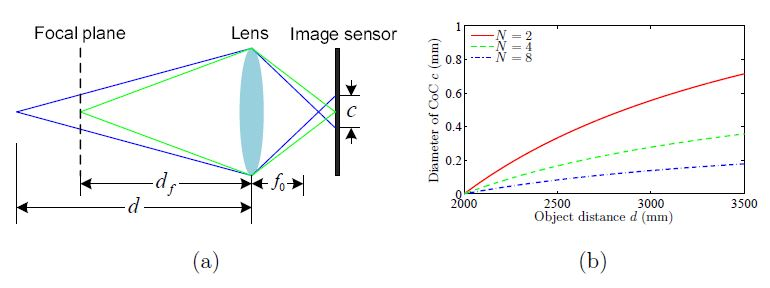
\includegraphics[width=1\linewidth]{pics/focus}
	\caption{Тонкая модель объектива}
	\label{fig:focus}
\end{figure}

где $f_0$ и $N$ - фокусное расстояние и номер остановки камеры соответственно. На рисунке~\ref{fig:focus} показаны фокус и расфокусировка для модели тонких линз и как изменяется диаметр круга замешательства с $d$ и $N$, при фиксированном $f_0$ и $d_f$.
Как мы видим, диаметр CoC $c$ является нелинейной монотонно возрастающей функцией расстояния объекта $d$. Размытие дефокусировки может быть смоделировано как свертка острого изображения с функцией распределения точек (PSF). PSF обычно аппроксимируется гауссовой функцией $g(x,\sigma)$, где стандартное отклонение $\sigma=kc$ пропорционально диаметру CoC $c$. Используем $\sigma$ как меру глубины сцены. Следовательно, размытие ребра $i(x)$ можно представить следующим образом,

\begin{equation}\label{eq:3}
i(x)=f(x)\otimes g(x,\sigma)
\end{equation}

\subsection{Оценка размытости}

На рисунке~\ref{fig:blur} показан обзор метода оценки размытия. Граница шага повторно размыта с использованием гауссова ядра с известным стандартным отклонением. затем рассчитывается соотношение между величиной градиента края ступени и ее размытой версией. Это максимальное значение в краевом положении. Используя максимальное значение, можем вычислить величину размытости дефокусировки в местоположении края.

\begin{figure}[H]
	\centering
	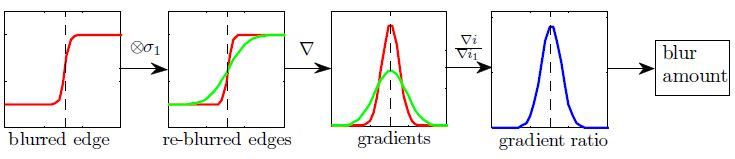
\includegraphics[width=1\linewidth]{pics/blur}
	\caption{Оценка размытости, черная штриховая линия обозначает местоположение края}
	\label{fig:blur}
\end{figure}

Используем двумерное изотропное гауссовское ядро для повторного размытия и величину градиента можно вычислить следующим образом:

\begin{equation}\label{eq:4}
||\bigtriangledown i(x,y)||=\sqrt{\bigtriangledown i_x^2+\bigtriangledown i_y^2}
\end{equation}

где $\bigtriangledown i_x$ и $\bigtriangledown i_y$- градиенты вдоль направлений x и y соответственно. Устанавливаем повторное размытие $\sigma_0=1$ и используем детектор края Canny ~\cite{IEEE} для выполнения обнаружения края.
Шкала размытия оценивается в каждом краевом положении, образуя редкую
карта глубины, обозначаемая $\hat{d}(x)$. Однако из-за шума или мягких теней оценки размытия могут содержать некоторые ошибки. Чтобы подавить эти ошибки, применяется совместный двусторонний фильтр ~\cite{ACM} на разреженной карте глубин $\hat{d}(x)$. Выход совместного двустороннего фильтра в каждом краевом положении х определяется как:

\begin{equation}\label{eq:5}
BF(\hat{d}(x))=\frac{1}{W(x)}\sum_{y\in N(x)}G_{\sigma s}(||x-y||)G_{\sigma r}(||I(x)-I(j)||)\hat{d}(y)
\end{equation}

где $W(x)$ - коэффициент нормировки, а $N(x)$ - окрестность точки x, заданная размером пространственного гауссовского фильтра $G_{\sigma s}$. Фильтрация выполняется только по краям. Совместный двусторонний фильтр корректирует некоторые ошибки в разреженной карте глубины и избегать распространения этих ошибок в интерполяции глубины, описанной в следующем разделе.


\subsection{Интерполяция глубины}

Данный метод оценки размытия дает разреженную карту глубин $d(x)$ с оценками глубины в местах краев. Чтобы получить полную карту глубины $d(x)$, необходимо распространить эти значения из местоположений краев на все изображение. Найдем регуляризованное отображение глубины $d(x)$, которое близко к разреженной карте глубин $d(x)$ в каждом краевом положении. Для этих задач обычно используются методы интерполяции с учетом края~\cite{ACM2}. Здесь применяется матирующий лапласиан~\cite{IEEE2} для выполнения интерполяции.
Мы переписываем разреженную карту глубин d (x) и полное отображение глубины d (x) в их векторной форме как d и d. Тогда проблему интерполяции глубины можно сформулировать как минимизирующую следующую функцию стоимости:


\subsection{Эксперименты}

\begin{figure}[H]
	\centering
	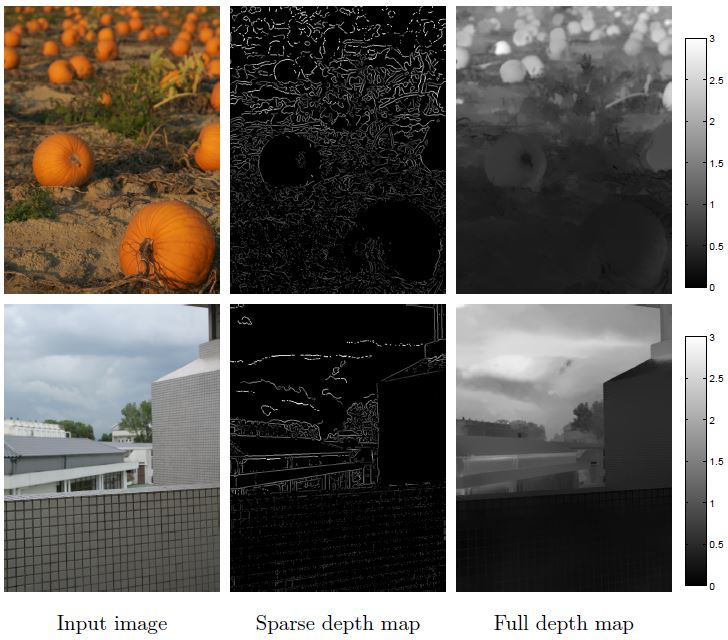
\includegraphics[width=0.7\linewidth]{pics/comparison}
	\caption{Восстановление глубины на реальных изображениях. Наш метод может работать как на сценах с непрерывной глубиной (изображение тыквы), так и на слоистой глубине (изображение здания) для получения карты глубины с довольно хорошей точностью.}
	\label{fig:comparison}
\end{figure}\

Как показано на рисунке~\ref{fig:comparison}, я тестирую наш метод на некоторых реальных изображениях. В изображении тыквы глубина сцены непрерывно изменяется от нижней к верхней части изображения. Оценочная карта глубины фиксирует непрерывное изменение глубины. В изображении здания сцена в основном содержит три слоя: стены, дом и небо. Наш метод позволяет создавать карты глубин, точно представляющие эти слои глубины. Как видно из результатов, наш метод позволяет точно восстановить глубину сцены из одного расфокусированного изображения. На рисунке~\ref{fig:flower} мы сравниваем наш метод с методом обратной диффузии~\cite{Proc}.

\begin{figure}[H]
	\centering
	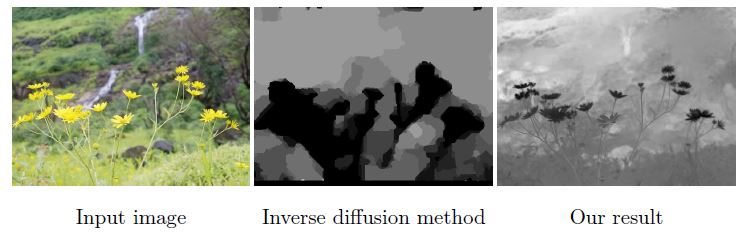
\includegraphics[width=1\linewidth]{pics/flower}
	\caption{Сравнение нашего метода с методом обратной диффузии, на примере цветка}
	\label{fig:flower}
\end{figure}\

Метод обратной диффузии создает грубую слоистую карту глубины. В результате этого цветочный слой плохо отделен фоновыми слоями и содержит некоторые оценки погрешности. Напротив, наш метод способен производить более точную и непрерывную карту глубины, а цветочный слой хорошо отделен фоновой травой и деревьями.